% ============================================================
%  Ramanalyze : Guide à l'usage des bénévoles
%  Niveau : débutant complet
% ============================================================

\documentclass[12pt, a4paper]{article}

% ── Encodage et langue ───────────────────────────────────────
\usepackage[utf8]{inputenc}
\usepackage[T1]{fontenc}
\usepackage[french]{babel}

% ── Mise en page ─────────────────────────────────────────────
\usepackage[top=2.5cm, bottom=2.8cm, left=2.8cm, right=2.8cm]{geometry}
\usepackage{parskip}
\usepackage{microtype}
\usepackage{lmodern}
\usepackage{setspace}
\setstretch{1.15}

% ── Couleurs ─────────────────────────────────────────────────
\usepackage{xcolor}
\definecolor{mainblue}{RGB}{25, 90, 160}
\definecolor{accentteal}{RGB}{20, 140, 130}
\definecolor{warnorange}{RGB}{210, 100, 20}
\definecolor{tipgreen}{RGB}{40, 140, 75}
\definecolor{stepbg}{RGB}{235, 242, 252}
\definecolor{figbg}{RGB}{225, 232, 240}
\definecolor{lightgray}{RGB}{245, 246, 248}
\definecolor{darkgray}{RGB}{80, 85, 95}
\definecolor{rulecolor}{RGB}{185, 195, 215}
% Dégradé onglets jaune-vert → vert
\definecolor{tab1col}{RGB}{188, 224, 60}
\definecolor{tab2col}{RGB}{135, 205, 55}
\definecolor{tab3col}{RGB}{78, 178, 60}
\definecolor{tab4col}{RGB}{46, 152, 62}
\definecolor{tab5col}{RGB}{26, 122, 52}
\definecolor{wflight}{RGB}{155, 215, 170}

% ── Graphique, figures et TikZ ────────────────────────────────
\usepackage{graphicx}
\usepackage{float}
\usepackage{tikz}
\usetikzlibrary{positioning, shapes.geometric, calc}

% ── Encadrés (tcolorbox) ─────────────────────────────────────
\usepackage{tcolorbox}
\tcbuselibrary{skins, breakable}

\newtcolorbox{conseil}{
  enhanced, breakable,
  colback=tipgreen!8!white, colframe=tipgreen!65!black,
  left=6pt, right=6pt, top=4pt, bottom=4pt,
  arc=4pt, boxrule=0.7pt,
  title={\small\bfseries Conseil},
  fonttitle=\small\bfseries,
  attach boxed title to top left={yshift=-2pt, xshift=6pt},
  boxed title style={colback=tipgreen!65!black, colframe=tipgreen!65!black,
                     arc=3pt, boxrule=0pt},
}

\newtcolorbox{attention}{
  enhanced, breakable,
  colback=warnorange!8!white, colframe=warnorange!75!black,
  left=6pt, right=6pt, top=4pt, bottom=4pt,
  arc=4pt, boxrule=0.7pt,
  title={\small\bfseries À noter},
  fonttitle=\small\bfseries,
  attach boxed title to top left={yshift=-2pt, xshift=6pt},
  boxed title style={colback=warnorange!75!black, colframe=warnorange!75!black,
                     arc=3pt, boxrule=0pt},
}

\newtcolorbox{enresume}{
  enhanced, breakable,
  colback=mainblue!6!white, colframe=mainblue!55!black,
  left=6pt, right=6pt, top=4pt, bottom=4pt,
  arc=4pt, boxrule=0.7pt,
  title={\small\bfseries En résumé},
  fonttitle=\small\bfseries,
  attach boxed title to top left={yshift=-2pt, xshift=6pt},
  boxed title style={colback=mainblue!55!black, colframe=mainblue!55!black,
                     arc=3pt, boxrule=0pt},
}

% ── Listes ───────────────────────────────────────────────────
\usepackage{enumitem}
\setlist[enumerate]{itemsep=3pt, parsep=0pt, topsep=4pt}
\setlist[itemize]{itemsep=3pt, parsep=0pt, topsep=4pt}

% ── Titres de sections ────────────────────────────────────────
\usepackage[explicit]{titlesec}

\titleformat{\section}
  {\normalfont\large\bfseries\color{mainblue}}
  {\thesection}
  {0.7em}
  {#1}
  [\vspace{2pt}{\color{rulecolor}\rule{\linewidth}{0.8pt}}\vspace{2pt}]

\titleformat{\subsection}
  {\normalfont\normalsize\bfseries\color{accentteal}}
  {\thesubsection}
  {0.5em}
  {#1}

\titleformat{\subsubsection}
  {\normalfont\normalsize\bfseries\color{darkgray}}
  {\thesubsubsection}
  {0.5em}
  {#1}

\titlespacing*{\section}{0pt}{14pt}{6pt}
\titlespacing*{\subsection}{0pt}{10pt}{4pt}

% ── En-tête et pied de page ───────────────────────────────────
\usepackage{fancyhdr}
\pagestyle{fancy}
\fancyhf{}
\renewcommand{\headrulewidth}{0pt}
\fancyhead[L]{\small\color{darkgray}\textit{Ramanalyze : Guide bénévoles}}
\fancyhead[R]{\small\color{darkgray}\thepage}
\fancyfoot[C]{\small\color{darkgray}\textit{CitizenSers : Usage interne}}

% ── Hyperliens ────────────────────────────────────────────────
\usepackage[hidelinks, colorlinks=true,
            linkcolor=mainblue, urlcolor=accentteal]{hyperref}

% ──────────────────────────────────────────────────────────────
%  Commandes personnalisées
% ──────────────────────────────────────────────────────────────

% Numéro d'étape dans un cercle coloré (utilisable dans le texte)
\newcommand{\numcercle}[1]{%
  \tikz[baseline=(n.base)]{%
    \node[circle, fill=mainblue, text=white,
          inner sep=2.5pt, font=\bfseries\small] (n) {#1};}%
}

% En-tête d'étape numérotée
\newcommand{\etape}[2]{%
  \vspace{10pt}%
  \noindent\numcercle{#1}\enskip
  {\large\bfseries\color{mainblue}#2}\par
  \vspace{3pt}%
  \noindent{\color{rulecolor}\rule{\linewidth}{0.4pt}}\par
  \vspace{4pt}%
}

% Représentation visuelle d'un bouton logiciel
\newcommand{\bouton}[1]{%
  \tikz[baseline=(b.base)]{%
    \node[rounded corners=3pt, fill=darkgray!12, draw=darkgray!35,
          inner xsep=5pt, inner ysep=2pt,
          font=\small\bfseries\color{darkgray}] (b) {#1};}%
}

% Nom d'un onglet
\newcommand{\onglet}[1]{\textbf{\color{mainblue}#1}}

% Nom d'un champ de saisie
\newcommand{\champ}[1]{\textit{\color{accentteal}\og\,#1\,\fg{}}}

% Capture d'écran réelle (width optionnel, nom de fichier, légende)
\newcommand{\figreal}[3][\linewidth]{%
  \begin{figure}[H]
    \centering
    {\setlength{\fboxsep}{0pt}\setlength{\fboxrule}{0.5pt}%
     \fbox{\includegraphics[width=#1]{Ramanalyze_visuel/#2}}}
    \caption{#3}
  \end{figure}%
}

% Capture pleine largeur (déborde légèrement sur les marges)
\newcommand{\figbig}[2]{%
  \begin{figure}[H]
    \makebox[\linewidth][c]{%
      \setlength{\fboxsep}{0pt}\setlength{\fboxrule}{0.5pt}%
      \fbox{\includegraphics[width=\dimexpr\linewidth+3.2cm\relax]{Ramanalyze_visuel/#1}}%
    }
    \caption{#2}
  \end{figure}%
}

% Placeholder de capture d'écran
\newcommand{\figph}[2][Capture d'écran]{%
  \begin{figure}[H]
    \centering
    \begin{tikzpicture}
      \node[
        draw=rulecolor,
        fill=figbg,
        rounded corners=5pt,
        minimum width=0.92\linewidth,
        minimum height=4.8cm,
        align=center,
        text width=0.82\linewidth,
        font=\small\color{darkgray}
      ] {%
        {\large\bfseries\color{rulecolor!70!darkgray}%
         \MakeUppercase{[ capture d'écran ]}}\\[8pt]
        #2%
      };
    \end{tikzpicture}
    \caption{#1}
  \end{figure}%
}

% ──────────────────────────────────────────────────────────────
\begin{document}

% ── Page de titre ─────────────────────────────────────────────
\begin{titlepage}
  \centering
  \vspace*{1cm}

  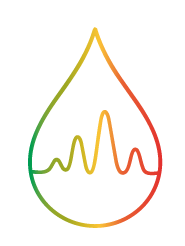
\includegraphics[width=0.3\linewidth]{../Logo Ramanalyze/logo ramanalyze.pdf}

  \vspace{1.2cm}

  {\Huge\bfseries\color{tab5col} Ramanalyze}\\[8pt]
  {\large\color{darkgray} Guide à l'usage des bénévoles}

  \vspace{1.2cm}
  {\large\color{darkgray}
    Comment analyser vos expériences Raman, pas à pas.}

  \vspace{0.4cm}
  {\normalsize\color{darkgray}
    Aucune connaissance en programmation ou en spectroscopie requise.}

  \vspace{1.8cm}

  \begin{figure}[H]
    \centering
    {\setlength{\fboxsep}{0pt}\setlength{\fboxrule}{0.5pt}%
     \fbox{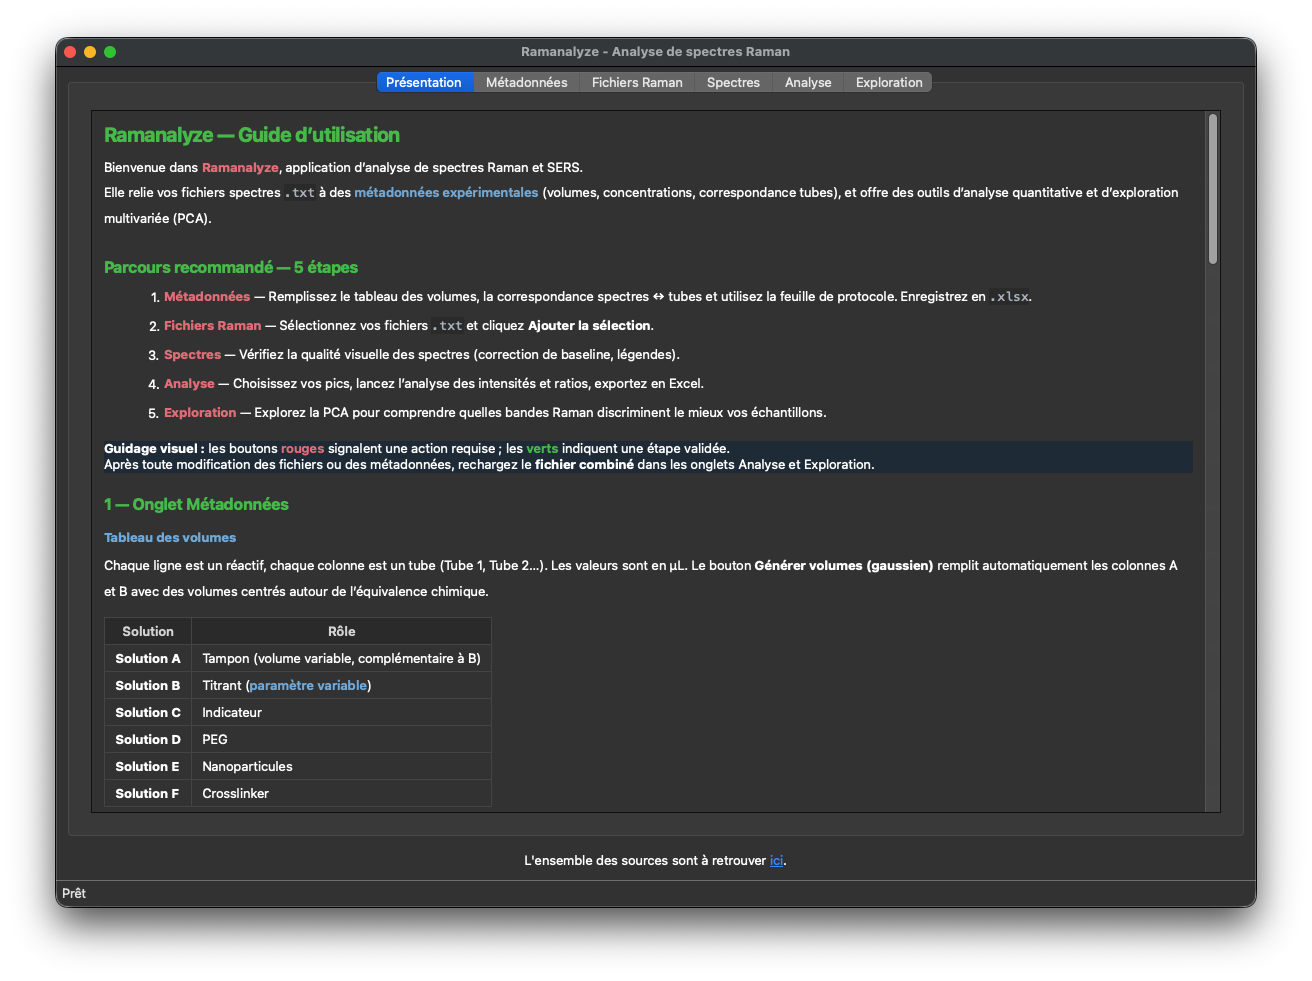
\includegraphics[width=1\linewidth]{Ramanalyze_visuel/Ramanalyze - ecran accueil .png}}}
    \caption{Vue générale du logiciel ouvert, avec les cinq onglets visibles en haut de la fenêtre.}
  \end{figure}

  \vfill

  {\color{darkgray}\small
    \textbf{CitizenSers} : Document à usage interne\\[6pt]
    Pour toute question, contactez la personne responsable
    de l'expérience.
  }
\end{titlepage}

\newpage
\tableofcontents
\newpage

% ══════════════════════════════════════════════════════════════
\section{Avant de commencer}
% ══════════════════════════════════════════════════════════════

\subsection{Ce que l'on mesure}
On utilise la spectroscopie Raman pour mesurer la quantité de cuivre contenue dans un échantillon d'eau prélevé dans l'environnement. Pour cela, 
un laser éclaire l'échantillon. La lumière renvoyée est analysée et
produit un \textbf{spectre Raman} : un graphique représentant l'intensité
lumineuse en fonction du nombre d'onde (en cm$^{-1}$). 

En gros, la lumière est composée de différentes longueurs d'onde (correspondant à différentes couleurs).
Le laser est composé, lui,  d'une seule longueur d'onde. Cependant, quand il traverse un échantillon liquide, il interagit avec les molécules présentes.
En intéragissant, certain faisceaux en parti modifié : leur longueur d'onde change légèrement (et donc leur nombre d'onde qui n'est autre que 1/longueur d'onde).
On peut voir ça comme une boule de flipper qui rebondit sur des obstacles : lors de certains rebonds, la boule perd un peu d'énergie (ou en regagne sur certain bonus). Son énergie est modifiée. 
Ainsi, en fonction de comment la lumière à été modifiée, on peut en déduire des informations sur les molécules présentes dans la solution.
C'est en quelque sorte une signature lumineuse propre à chaque molécule.

Au final, chaque molécule entraine un signal lumineux spécifiques à des valeurs précises, appelées
\textbf{pics}. 
On peut ensuite comparer l'intensité de deux pics en calculant un
\textbf{ratio} : c'est lui que l'on suit tout au long de l'expérience.

Dans notre cas, on cherche à mesurer la quantité de cuivre présente dans
un échantillon d'eau. Pour cela, on réalise une \textbf{titration} : on
ajoute progressivement une solution dont on connaît la concentration, et on
observe comment le ratio évolue. À un moment précis, les deux espèces
chimiques se trouvent en quantités égales : c'est le \textbf{point
d'équivalence}. A ce point, le ratio des deux deux pics suivi évolue drastiquement, et c'est ainsi qu'on peut le repérer.
 En connaissant la quantité ajoutée à ce moment-là, on peut
déduire la quantité de cuivre initialement présente dans l'échantillon.

Le tout est maintenant de trouver ce point d'équivalence à partir des spectres acquis : c'est ce que le logiciel \textbf{Ramanalyze} vous aide à faire, étape par étape.

\begin{conseil}
  Inutile de comprendre la physique exacte du Raman pour utiliser ce logiciel.
  L'idéal est d'avoir compris notre objectif, l'idée de la méthode et comment techniquement on l'atteint (acquisition puis analyse).
  Ensuite, il suffit de suivre les étapes dans l'ordre.
\end{conseil}

\subsection{Ce que fait le logiciel}

Ramanalyze rassemble en un seul endroit toutes les tâches d'analyse.

\begin{enumerate}
  \item Il permet de saisir les informations de l'expérience (concentrations, volumes, correspondance spectre / tube).
  \item Il intégre les feuilles de remplissage des volumes, et permets un suivi détaillé à la paillasse.
  \item Il lit les fichiers bruts produits par le spectromètre.
  \item Il les associe aux informations de l'expérience (concentrations,
        volumes, correspondance spectre / tube).
  \item Il trace les spectres pour les visualiser.
  \item Il calcule les ratios d'intensité entre les pics et trace leur
        évolution en fonction de la quantité de titrant.
  \item Il ajuste une courbe mathématique pour localiser le point
        d'équivalence.
  \item Il exporte les résultats dans un fichier Excel.
\end{enumerate}

\subsection{Les cinq onglets}

Le logiciel est organisé en cinq onglets, affichés en haut de la fenêtre.
On les parcourt \textbf{de gauche à droite} lors d'une nouvelle analyse.

\begin{center}
\begin{tikzpicture}[node distance=0.2cm]
  \node[rounded corners=3pt, fill=tab1col, draw=tab1col!70!black,
        minimum width=2.6cm, minimum height=0.75cm,
        font=\small\bfseries\color{tab5col}]
        (t1) {Présentation};
  \node[rounded corners=3pt, fill=tab2col, draw=tab2col!70!black,
        minimum width=2.6cm, minimum height=0.75cm,
        font=\small\bfseries\color{white},
        right=of t1] (t2) {Métadonnées};
  \node[rounded corners=3pt, fill=tab3col, draw=tab3col!70!black,
        minimum width=2.6cm, minimum height=0.75cm,
        font=\small\bfseries\color{white},
        right=of t2] (t3) {\small Fichiers Raman};
  \node[rounded corners=3pt, fill=tab4col, draw=tab4col!70!black,
        minimum width=2.6cm, minimum height=0.75cm,
        font=\small\bfseries\color{white},
        right=of t3] (t4) {Spectres};
  \node[rounded corners=3pt, fill=tab5col, draw=tab5col!70!black,
        minimum width=2.6cm, minimum height=0.75cm,
        font=\small\bfseries\color{white},
        right=of t4] (t5) {Analyse};

  \draw[->, thick, color=tab3col] (t1.east) -- (t2.west);
  \draw[->, thick, color=tab3col] (t2.east) -- (t3.west);
  \draw[->, thick, color=tab3col] (t3.east) -- (t4.west);
  \draw[->, thick, color=tab3col] (t4.east) -- (t5.west);
\end{tikzpicture}
\end{center}

\vspace{6pt}
\begin{itemize}
  \item \onglet{Présentation} : informations générales sur le logiciel.
        Rien à faire ici lors d'une analyse.
  \item \onglet{Métadonnées} : saisie des informations de l'expérience
        (nom, concentrations, volumes) et export de la feuille de
        protocole de paillasse. Dans cet onglet, vous pouvez à la fois gérer votre protocole à venir, 
        et/ou saisir les informations d'une expérience déjà réalisée.
  \item \onglet{Fichiers Raman} : chargement des fichiers spectres bruts
        et génération du fichier de travail.
  \item \onglet{Spectres} : visualisation des spectres acquis.
  \item \onglet{Analyse} : calcul des ratios, ajustement de courbe et
        export des résultats.
\end{itemize}

\figbig{vis-accueil.png}{Vue générale du logiciel : les cinq onglets sont visibles en haut de la fenêtre.}

\newpage

% ══════════════════════════════════════════════════════════════
\section{Étape 1 : Renseigner les informations de l'expérience}
% ══════════════════════════════════════════════════════════════

\subsection{Objectif}

Avant d'analyser les spectres, le logiciel a besoin de connaître le
protocole expérimental : nombre de tubes, concentrations et volumes
des solutions utilisées.
Ces informations sont appelées les \textbf{métadonnées}.

Cette étape demande un peu plus de soin, mais elle n'est à réaliser
qu'une seule fois par expérience.
Vous n'avez pas encore besoin des fichiers spectres à ce stade.

\subsection{Ouvrir l'onglet Métadonnées}

Cliquez sur l'onglet \onglet{Métadonnées}.

\figbig{vis-metadonnees.png}{Vue générale de l'onglet Métadonnées : informations générales, boutons de gestion des tableaux et boutons de sauvegarde.}

\subsection{Informations générales}

\etape{1}{Renseigner le nom de la manipulation}

Cliquez dans le champ \champ{Nom de la manipulation} et tapez
l'identifiant de votre expérience.
Exemple : \texttt{GC001}.

\etape{2}{Décrire l'échantillon}

Remplissez le champ \champ{Sample description}.
Exemple : \texttt{Cuivre 1\,µM, EGTA, tampon pH\,7}.

Ce texte servira de légende dans les graphiques.

\etape{3}{Vérifier la longueur d'onde du laser}

Assurez-vous que la valeur affichée correspond au laser utilisé lors
de l'acquisition (532\,nm ou 785\,nm en général).

\figbig{vis-metadonnees-vertes.png}{Onglet Métadonnées avec les informations renseignées : les boutons passent au vert une fois les tableaux complétés.}

\subsection{Générer le tableau des volumes}

Le tableau des volumes liste le volume de chaque réactif à pipeter
dans chaque tube.
Le logiciel peut le calculer automatiquement à partir de votre
protocole.

\etape{4}{Ouvrir le dialogue de génération}

Cliquez sur \bouton{Créer / éditer le tableau des volumes}.
Une fenêtre s'ouvre.

\figreal[0.6\linewidth]{vis-generation-volume.png}{Dialogue de génération des volumes : paramètres principaux, solutions fixes et options avancées.}

\etape{5}{Renseigner les paramètres principaux}

Ces valeurs se trouvent dans votre protocole de paillasse.

\begin{itemize}
  \item \champ{Nombre de tubes} : nombre total de tubes dans
        l'expérience.
  \item \champ{C0 Cu (nM)} : concentration initiale de cuivre dans
        l'échantillon pur, en nanomolaires.
  \item \champ{V échantillon (µL)} : volume d'échantillon par tube,
        en microlitres.
  \item \champ{C titrant (µM)} : concentration de la solution titrante
        (Solution B), en micromolaires.
  \item \champ{V total par tube (µL)} : volume final souhaité dans
        chaque tube.
\end{itemize}

\begin{conseil}
  En cas de doute sur une valeur, demandez à la personne responsable
  de l'expérience avant de continuer.
\end{conseil}

\etape{6}{Renseigner les solutions fixes C, D, E, F}

Si votre protocole utilise des solutions supplémentaires (tampon, sel,
ligand), renseignez pour chacune :

\begin{itemize}
  \item \champ{Volume (µL)} : volume à pipeter dans chaque tube.
  \item \champ{Concentration} : concentration du stock, dans l'unité
        indiquée à droite (M, mM, µM, nM ou \% en masse).
\end{itemize}

\begin{attention}
  Le volume et la concentration sont des champs indépendants.
  Modifier l'un ne modifie pas l'autre automatiquement.
  Vérifiez bien les deux.
\end{attention}

\etape{7}{Mode compte-goutte (si applicable)}

Si vous utilisez un \textbf{compte-goutte} (chaque goutte vaut
environ 40\,µL), cochez la case
\champ{Utilisation d'un compte-goutte}.
Le logiciel pré-remplit les paramètres adaptés.
Vous pouvez ensuite modifier chaque valeur si besoin.

Si vous utilisez une pipette classique, laissez cette case décochée.

\etape{8}{Valider et fermer}

Cliquez sur \bouton{OK}.
Le tableau des volumes s'affiche dans l'onglet Métadonnées.

\figreal{vis-tableau-volume.png}{Tableau des volumes : chaque colonne est un tube, chaque ligne un réactif. La ligne verte en bas indique le volume total.}

\begin{conseil}
  Vous pouvez corriger n'importe quelle valeur en double-cliquant
  sur la cellule correspondante.
\end{conseil}

\subsection{Exporter la feuille de protocole}

Le logiciel peut générer une \textbf{feuille de protocole} au format
Excel, prête à imprimer et à utiliser à la paillasse.
Elle récapitule, pour chaque réactif et chaque tube, le volume exact
à prélever, avec des cases à cocher pour le coordinateur et
l'opérateur.

\etape{9}{Générer la feuille de protocole}

\begin{enumerate}
  \item Cliquez sur \bouton{Feuille de protocole\ldots}.
  \item Vous avez la possibilité de le remplir directement sur le logiciel, ou de l'imprimer pour le remplir à la main.
  \item Cliqué sur \bouton{Exporter Excel\ldots}.
  \item Choisissez un emplacement et un nom de fichier.
        Exemple : \texttt{GC001\_protocole}.
  \item Cliquez sur \bouton{Enregistrer}.
\end{enumerate}

\figbig{Ramanalyze - feuille excel suivi en remplissage.png}{Feuille de protocole Excel générée — en cours de remplissage à la paillasse.}

\figbig{Ramanalyze - feuille excel suivi remplie.png}{Feuille de protocole Excel générée — complètement remplie.}

\begin{conseil}
  Cette feuille est particulièrement utile en binôme à la paillasse :
  le coordinateur annonce les volumes pendant que l'opérateur pipete
  et coche les cases au fur et à mesure. Ces cases sont des gardes fous pour éviter des erreurs sur les volumes introduits et assurer une expériences réussie.
\end{conseil}

\subsection{Enregistrer les métadonnées}

\etape{10}{Sauvegarder}

\begin{enumerate}
  \item Cliquez sur \bouton{Enregistrer les métadonnées\ldots}.
  \item Choisissez un dossier et un nom de fichier.
        Exemple : \texttt{GC001\_metadonnees}.
  \item Cliquez sur \bouton{Enregistrer}.
\end{enumerate}

Le fichier est sauvegardé au format Excel (\texttt{.xlsx}).
Vous pourrez le recharger lors d'une session ultérieure.

\begin{conseil}
  Enregistrez les métadonnées \textbf{avant} de passer à l'onglet
  suivant. Si vous fermez le logiciel sans sauvegarder, toutes les
  informations saisies seront perdues.
\end{conseil}

\begin{enresume}
  À l'issue de cette étape, les informations générales et le tableau
  des volumes sont saisis et sauvegardés.
  La feuille de protocole est prête à imprimer si vous en avez besoin
  à la paillasse.
  Le tableau de correspondance spectres\,/\,tubes sera complété à
  l'étape suivante, une fois les fichiers Raman chargés.
\end{enresume}

\newpage

% ══════════════════════════════════════════════════════════════
\section{Étape 2 : Charger les fichiers Raman}
% ══════════════════════════════════════════════════════════════

\subsection{Objectif}

Charger dans le logiciel les fichiers produits par le spectromètre,
puis compléter le tableau de correspondance qui relie chaque fichier
spectre à son tube.

\subsection{Charger les spectres}

\etape{1}{Ouvrir l'onglet Fichiers Raman}

Cliquez sur l'onglet \onglet{Fichiers Raman} en haut de la fenêtre.

\figbig{vis-fichiers-raman.png}{Onglet Fichiers Raman avec des fichiers sélectionnés dans le panneau gauche : les fichiers validés apparaissent à droite.}

\etape{2}{Ajouter les fichiers de l'expérience}

\begin{enumerate}
  \item Dans le panneau gauche, naviguez jusqu'au dossier contenant
        les fichiers de votre expérience.
  \item Pour sélectionner tous les fichiers en une seule fois, cliquez
        sur le premier fichier de la liste, puis maintenez la touche
        \textbf{Maj} (\texttt{Shift}) enfoncée et cliquez sur le dernier.
        Tous les fichiers intermédiaires sont sélectionnés.
  \item Cliquez sur \bouton{Ajouter la sélection}.
        Les fichiers apparaissent dans le panneau de droite.
\end{enumerate}

\begin{attention}
  Sélectionnez uniquement les fichiers \texttt{.txt} de votre
  expérience.
  Ajouter des fichiers d'une autre manipulation risquerait de vous
  induire en erreur par la suite.
\end{attention}

\etape{3}{Vérifier la liste}

Les fichiers ajoutés apparaissent dans la liste.
Vérifiez avoir bien sélectionné l'ensemble des spectres acquis que
vous souhaitez analyser.

Pour retirer un fichier ajouté par erreur, cliquez dessus pour le
sélectionner, puis cliquez sur \bouton{Retirer}.

\begin{conseil}
  Si vous avez acquis plusieurs spectres par tube (deux réplicats par
  exemple), chargez tous les fichiers correspondants.
\end{conseil}

\figbig{vis-fichier-raman-full.png}{Onglet Fichiers Raman avec les fichiers chargés dans la liste de droite, prêts à être analysés.}

\subsection{Remplir le tableau de correspondance}

Le tableau de correspondance indique \textbf{quel fichier spectre
correspond à quel tube}.
Sans cette information, le logiciel ne peut pas relier les données
spectroscopiques aux concentrations.

\etape{4}{Revenir à l'onglet Métadonnées}

Cliquez sur l'onglet \onglet{Métadonnées}.
Le tableau de correspondance se trouve en bas de la page.

\etape{5}{Comprendre le tableau}

Le tableau comporte deux colonnes principales.

\begin{itemize}
  \item La colonne de gauche liste les fichiers spectres que vous venez
        de charger.
  \item La colonne de droite indique le numéro du tube associé.
\end{itemize}

\etape{6}{Associer chaque spectre à son tube}

\begin{enumerate}
  \item Cliquez sur la cellule de la colonne \champ{Tube} en face du
        fichier spectre concerné.
  \item Tapez le numéro du tube correspondant.
  \item Répétez pour chaque ligne.
\end{enumerate}

\figreal[0.72\linewidth]{vis-correspondances.png}{Tableau de correspondance spectres\,/\,tubes : chaque fichier spectre est associé à un numéro de tube.}

\begin{attention}
  Si vous avez acquis deux réplicats pour un même tube, les deux
  fichiers doivent recevoir le même numéro de tube.
\end{attention}

\etape{7}{Sauvegarder les métadonnées complètes}

\begin{enumerate}
  \item Cliquez sur \bouton{Enregistrer les métadonnées\ldots}.
  \item Vérifiez que le nom de fichier correspond bien à votre
        expérience (exemple : \texttt{GC001\_metadonnees}).
  \item Cliquez sur \bouton{Enregistrer}.
\end{enumerate}

\begin{enresume}
  À l'issue de cette étape, tous les fichiers spectres sont chargés
  et chaque spectre est associé à son tube.
  Le logiciel dispose de toutes les informations pour lancer l'analyse.
\end{enresume}

\newpage

% ══════════════════════════════════════════════════════════════
\section{Étape 3 : Visualiser les spectres}
% ══════════════════════════════════════════════════════════════

\subsection{Objectif}

Afficher les spectres pour vérifier qu'ils ont bien été acquis et
qu'aucun ne présente d'anomalie (bruit excessif, pic manquant,
ligne de base incohérente).

\subsection{Procédure}

\etape{1}{Ouvrir l'onglet Spectres}

Cliquez sur l'onglet \onglet{Spectres}.

\etape{2}{Tracer les spectres}

Cliquez sur \bouton{Tracer avec baseline}.

Le graphique s'affiche en quelques secondes.
Chaque courbe correspond à un spectre.
Les couleurs permettent de les distinguer.

\figbig{vis-spectres.png}{Onglet Spectres : les spectres de chaque tube sont superposés et colorés. La légende à droite identifie chaque courbe.}

\subsection{Naviguer dans le graphique}

Le graphique est interactif.

\begin{itemize}
  \item \textbf{Zoomer} : maintenez le clic gauche et dessinez un
        rectangle sur la zone à agrandir.
  \item \textbf{Se déplacer} : maintenez le clic gauche et faites
        glisser le graphique.
  \item \textbf{Revenir à la vue complète} : double-cliquez sur le
        graphique, ou cliquez sur l'icône en forme de maison dans la
        barre d'outils en haut à droite.
  \item \textbf{Masquer une courbe} : cliquez sur son nom dans la
        légende.
        Cliquez à nouveau pour la faire réapparaître.
\end{itemize}

\figbig{vis-spectres-zoom.png}{Vue zoomée sur les pics principaux : la barre d'outils Plotly en haut à droite permet de zoomer, se déplacer ou revenir à la vue complète.}

\subsection{Exporter le graphique des spectres}

\begin{enumerate}
  \item Cliquez sur \bouton{Exporter le graphique\ldots}.
  \item Choisissez le \textbf{format} :
        PNG pour une image classique,
        SVG pour une image vectorielle (idéale pour publications),
        PDF pour un document prêt à imprimer.
  \item Choisissez la \textbf{taille} dans la liste déroulante.
        Pour un rapport ou une publication, choisissez
        \champ{A4 paysage (297$\times$210\,mm, 150\,dpi)}.
  \item Cliquez sur \bouton{OK}.
  \item Choisissez l'emplacement de sauvegarde et cliquez sur
        \bouton{Enregistrer}.
\end{enumerate}

\begin{conseil}
  Le format SVG est vectoriel : l'image reste parfaitement nette
  quelle que soit sa taille d'affichage ou d'impression.
  C'est le format recommandé pour les figures de publications.
\end{conseil}

\begin{enresume}
  À l'issue de cette étape, vous avez visualisé tous les spectres
  et vérifié leur qualité.
  Si un spectre vous semble anormal, notez son nom avant de
  passer à l'analyse.
\end{enresume}

\newpage

% ══════════════════════════════════════════════════════════════
\section{Étape 4 : Analyser les pics}
% ══════════════════════════════════════════════════════════════

\subsection{Objectif}

Demander au logiciel de mesurer automatiquement l'intensité à chaque
pic d'intérêt dans chaque spectre, de calculer les ratios entre ces
intensités, et de tracer leur évolution en fonction de la quantité de
titrant.
C'est l'étape centrale de l'analyse.

\subsection{Ouvrir l'onglet Analyse}

Cliquez sur l'onglet \onglet{Analyse}.

\figbig{vis-analyse-avant.png}{Onglet Analyse avant chargement du fichier combiné : les boutons principaux sont visibles en haut.}

\etape{1}{Recharger le fichier combiné si nécessaire}

Si vous reprenez une session après avoir fermé le logiciel, cliquez sur
\bouton{Recharger le fichier combiné depuis Métadonnées}.
Cela garantit que les dernières métadonnées sont bien prises en compte.

\subsection{Choisir le jeu de pics}

\etape{2}{Sélectionner le jeu adapté à votre laser}

Dans la liste \champ{Jeu de pics}, choisissez :

\begin{itemize}
  \item \champ{532\,nm : paires pré-enregistrées} : pour un laser
        à 532\,nm. C'est le choix le plus courant.
  \item \champ{785\,nm} : pour un laser à 785\,nm.
  \item \champ{Personnalisé} : si vous souhaitez saisir vos propres
        nombres d'onde, entrez-les dans le champ \champ{Pics à étudier},
        séparés par des virgules.
        Exemple : \texttt{1234, 1364, 1580}.
\end{itemize}

\etape{3}{Vérifier la tolérance}

Le champ \champ{Tolérance (cm$^{-1}$)} définit la marge de recherche
autour de chaque pic.
La valeur par défaut (5,00\,cm$^{-1}$) convient dans la grande
majorité des cas.
Ne la modifiez pas sauf indication contraire.

\figbig{vis-analyse-chargee.png}{Onglet Analyse avec le fichier combiné chargé : le bouton \og Recharger \fg{} passe au vert, indiquant que les données sont prêtes.}

\subsection{Lancer l'analyse}

\etape{4}{Cliquer sur Analyser les pics}

Cliquez sur \bouton{Analyser les pics}.

Le logiciel effectue les opérations suivantes.

\begin{enumerate}
  \item Il recherche l'intensité maximale autour de chaque pic dans
        chaque spectre.
  \item Il calcule tous les ratios possibles entre ces intensités.
  \item Il associe chaque spectre à son tube et à la quantité de
        titrant correspondante.
  \item Il affiche un tableau de résultats et le graphique des ratios.
\end{enumerate}

\figbig{vis-analyse-faites.png}{Résultat de l'analyse : le graphique des rapports d'intensité Raman affiche l'évolution de chaque ratio en fonction de la quantité de titrant.}

\begin{conseil}
  Si le calcul prend quelques secondes, c'est normal.
  Attendez sans fermer le logiciel.
\end{conseil}

\subsection{Ajuster une courbe sigmoïde}

Pour localiser précisément le \textbf{point d'équivalence}, on ajuste
une courbe en forme de S (sigmoïde) sur le ratio de son choix.

\etape{5}{Sélectionner le ratio à ajuster}

Dans la liste \champ{Ratio à ajuster}, choisissez le ratio dont la
courbe présente la variation la plus nette.

\etape{6}{Lancer l'ajustement}

Cliquez sur \bouton{Ajuster par sigmoïde}.
La courbe ajustée apparaît en pointillés sur le graphique.

\etape{7}{Afficher le point d'équivalence}

Cliquez sur \bouton{Afficher l'équivalence}.
La valeur du point d'équivalence s'affiche sur le graphique,
accompagnée d'une ligne verticale en pointillés.

\figbig{vis-analyse-sigmoide.png}{Ajustement sigmoïde sur le ratio sélectionné : le point d'équivalence est annoté sur le graphique avec sa valeur.}

\begin{attention}
  Si l'ajustement produit une courbe incohérente (qui ne passe pas par
  les points mesurés), cela indique généralement que ce ratio n'est
  pas le plus adapté.
  Essayez-en un autre dans la liste.
  Si le problème persiste, consultez la personne responsable.
\end{attention}

\subsection{Exporter les résultats}

\etape{8}{Exporter vers Excel}

\begin{enumerate}
  \item Cliquez sur \bouton{Exporter résultats (Excel)\ldots}.
  \item Choisissez un dossier et un nom.
        Exemple : \texttt{GC001\_resultats}.
  \item Cliquez sur \bouton{Enregistrer}.
\end{enumerate}

Le fichier Excel créé contient deux feuilles.

\begin{itemize}
  \item \texttt{intensites} : l'intensité mesurée à chaque pic,
        pour chaque spectre.
  \item \texttt{ratios} : tous les ratios calculés, avec les
        métadonnées associées (tube, concentration, quantité de
        titrant).
\end{itemize}

\etape{9}{Exporter le graphique}

\begin{enumerate}
  \item Cliquez sur \bouton{Enregistrer le graphique}.
  \item Choisissez le format (PNG, SVG ou PDF) et la taille de sortie.
  \item Cliquez sur \bouton{OK}.
  \item Choisissez l'emplacement de sauvegarde.
\end{enumerate}

\figreal[0.87\linewidth]{Ramanalyze-enregistrement graphique.png}
{Dialogue d'export du graphique : choix du format (PNG, SVG, PDF) et de la taille de sortie.
Par la suite, il vous sera demandé de choisir l'emplacement de sauvegarde et de cliquer sur \og Enregistrer \fg{}.}

\begin{enresume}
  À l'issue de cette étape, vous disposez des ratios d'intensité,
  des points d'équivalence et de tous les fichiers exportés.
  L'analyse est terminée.
\end{enresume}

\newpage

% ══════════════════════════════════════════════════════════════
\section{Récapitulatif du workflow}
% ══════════════════════════════════════════════════════════════

\begin{center}
\begin{tikzpicture}[node distance=0.45cm]

  \tikzstyle{stepbox} = [
    rounded corners=5pt,
    draw=none,
    minimum width=10.5cm, minimum height=1.1cm,
    align=left, text width=9.8cm,
    font=\small, text=white
  ]

  \node[stepbox, fill=tab5col] (s1)
    {{\bfseries 1.}\enskip
     Renseigner les informations générales (onglet \textbf{Métadonnées})};

  \node[stepbox, fill=tab5col!91!wflight, below=of s1] (s2)
    {{\bfseries 2.}\enskip
     Générer le tableau des volumes};

  \node[stepbox, fill=tab5col!82!wflight, below=of s2] (s3)
    {{\bfseries 3.}\enskip
     Exporter la feuille de protocole de paillasse (facultatif)};

  \node[stepbox, fill=tab5col!73!wflight, below=of s3] (s4)
    {{\bfseries 4.}\enskip
     Ou charger la feuille de protocole réalisée};

  \node[stepbox, fill=tab5col!64!wflight, below=of s4] (s5)
    {{\bfseries 5.}\enskip
     Charger les fichiers \texttt{.txt} (onglet \textbf{Fichiers Raman})};

  \node[stepbox, fill=tab5col!50!wflight, below=of s5] (s6)
    {{\bfseries 6.}\enskip
     Remplir le tableau de correspondance spectres\,/\,tubes};

  \node[stepbox, fill=tab5col!40!wflight, below=of s6] (s7)
    {{\bfseries 7.}\enskip
     Enregistrer les métadonnées complètes (\texttt{.xlsx})};

  \node[stepbox, fill=tab5col!30!wflight, below=of s7] (s8)
    {{\bfseries 8.}\enskip
     Visualiser et vérifier les spectres (onglet \textbf{Spectres})};

  \node[stepbox, fill=tab5col!20!wflight, below=of s8] (s9)
    {{\bfseries 9.}\enskip
     Analyser les pics (onglet \textbf{Analyse})};

  \node[stepbox, fill=tab5col!10!wflight, below=of s9] (s10)
    {{\bfseries 10.}\enskip
     Ajuster la sigmoïde et lire le point d'équivalence};

  \node[stepbox, fill=wflight, below=of s10] (s11)
    {{\bfseries 11.}\enskip
     Exporter les résultats Excel et le graphique};

  \draw[->, thick, color=tab5col!60!white] (s1.south) -- (s2.north);
  \draw[->, thick, color=tab5col!60!white] (s2.south) -- (s3.north);
  \draw[->, thick, color=tab5col!60!white] (s3.south) -- (s4.north);
  \draw[->, thick, color=tab5col!60!white] (s4.south) -- (s5.north);
  \draw[->, thick, color=tab5col!60!white] (s5.south) -- (s6.north);
  \draw[->, thick, color=tab5col!60!white] (s6.south) -- (s7.north);
  \draw[->, thick, color=tab5col!60!white] (s7.south) -- (s8.north);
  \draw[->, thick, color=tab5col!60!white] (s8.south) -- (s9.north);
  \draw[->, thick, color=tab5col!60!white] (s9.south) -- (s10.north);
  \draw[->, thick, color=tab5col!60!white] (s10.south) -- (s11.north);

\end{tikzpicture}
\end{center}

\newpage

% ══════════════════════════════════════════════════════════════
\section{Reprendre une session interrompue}
% ══════════════════════════════════════════════════════════════

Si vous avez fermé le logiciel en cours d'analyse, voici comment
reprendre exactement là où vous en étiez.

\begin{enumerate}
  \item Ouvrez le logiciel.
  \item Cliquez sur l'onglet \onglet{Métadonnées}.
  \item Cliquez sur \bouton{Charger des métadonnées\ldots}.
  \item Naviguez jusqu'au fichier \texttt{.xlsx} de métadonnées que
        vous avez enregistré précédemment et sélectionnez-le.
  \item Cliquez sur \bouton{Ouvrir}.
  \item Cliquez sur l'onglet \onglet{Fichiers Raman}.
  \item Rechargez les fichiers spectres comme indiqué à l'étape 2
        et régénérez le fichier combiné.
  \item Reprenez à l'étape interrompue.
\end{enumerate}

\begin{conseil}
  Enregistrez les métadonnées régulièrement.
  Vous ne perdez ainsi jamais les informations de votre expérience,
  même en cas de fermeture accidentelle du logiciel.
\end{conseil}

% ══════════════════════════════════════════════════════════════
\section{Questions fréquentes}
% ══════════════════════════════════════════════════════════════

\textbf{Le graphique des spectres est vide après avoir cliqué sur
\og Tracer avec baseline \fg{}.}

Vérifiez que le fichier combiné a bien été généré.
Si ce n'est pas le cas, retournez dans l'onglet
\onglet{Fichiers Raman} et cliquez à nouveau sur
\bouton{Générer le fichier combiné\ldots}.

\bigskip

\textbf{Le tableau de correspondance est vide ou incomplet.}

Retournez dans l'onglet \onglet{Métadonnées} et vérifiez que chaque
fichier spectre dispose d'un numéro de tube dans la colonne
\champ{Tube}.

\bigskip

\textbf{L'ajustement sigmoïde affiche un message d'erreur.}

Cela peut survenir lorsque le ratio sélectionné ne présente pas de
transition nette.
Choisissez un autre ratio dans la liste \champ{Ratio à ajuster}.
Si le problème persiste, consultez la personne responsable.

\bigskip

\textbf{Je veux remettre tous les paramètres à zéro dans le dialogue
des volumes.}

Dans le dialogue de génération des volumes, cliquez sur
\bouton{Valeurs par défaut}.
Cela remet tous les champs aux valeurs d'usine sans fermer la fenêtre.

\bigskip

\textbf{Je souhaite ajouter ou supprimer un tube dans le tableau des
volumes.}

Dans le dialogue du tableau des volumes, cliquez d'abord sur
l'en-tête de la colonne du tube concerné (ligne des titres) pour le
sélectionner, puis cliquez sur \bouton{Supprimer le tube sélectionné}
ou \bouton{Dupliquer le tube sélectionné} selon l'action souhaitée.

\bigskip

\textbf{L'export PDF ne ressemble pas à l'affichage dans le logiciel.}

Préférez l'export \textbf{PNG haute résolution} ou \textbf{SVG
vectoriel}, qui reproduisent exactement ce qui est affiché à l'écran.

\newpage

% ══════════════════════════════════════════════════════════════
% ANNEXE
% ══════════════════════════════════════════════════════════════

\appendix

\section{Pour aller plus loin : L'onglet Exploration}

\begin{tcolorbox}[
  enhanced, colback=warnorange!8!white, colframe=warnorange!65!black,
  left=6pt, right=6pt, top=4pt, bottom=4pt, arc=4pt, boxrule=0.7pt,
  title={\small\bfseries Pour qui est cette annexe ?},
  fonttitle=\small\bfseries,
  attach boxed title to top left={yshift=-2pt, xshift=6pt},
  boxed title style={colback=warnorange!65!black,
                     colframe=warnorange!65!black,
                     arc=3pt, boxrule=0pt}
]
  Cette annexe s'adresse à des personnes déjà familières des méthodes
  d'analyse multivariée telles que l'Analyse en Composantes Principales
  (ACP).
  Elle n'est pas nécessaire pour une analyse courante.
\end{tcolorbox}

\subsection{Présentation générale}

L'onglet \onglet{Exploration} regroupe des outils d'analyse avancée.
Il propose plusieurs sous-onglets accessibles via les boutons
en haut de la zone de contenu.

\figreal{vis-exploration.png}{Vue générale de l'onglet Exploration après analyse : les sous-onglets (PCA corrélée, Scores, Loadings, Scatter matrix\ldots) sont accessibles en haut.}

\subsection{Sélection des pics}

Avant d'utiliser les outils d'exploration, définissez les pics à
analyser.

\begin{enumerate}
  \item Entrez les nombres d'onde dans le champ dédié, séparés par
        des virgules.
  \item Définissez la tolérance.
  \item Cliquez sur \bouton{Valider la sélection de pics}.
\end{enumerate}

\subsection{Spectres normalisés}

Affiche tous les spectres après normalisation par leur norme
vectorielle.
Cela permet de comparer la forme des spectres indépendamment de
leur intensité absolue.

\subsection{Spectres superposés}

Affiche les spectres bruts superposés, sans normalisation.

\subsection{PCA corrélée}

Réalise une Analyse en Composantes Principales sur les intensités
aux pics sélectionnés.
Chaque point représente un spectre.
La couleur indique la concentration de titrant.
Une séparation nette des points peut traduire un changement
structural dans l'échantillon.

\subsection{PCA libre (Scores, Loadings, Reconstruction)}

Ces sous-onglets réalisent une ACP sur l'ensemble du spectre et non
uniquement sur les pics sélectionnés.

\begin{itemize}
  \item \textbf{Scores} : position de chaque spectre dans l'espace
        des composantes principales.
  \item \textbf{Loadings} : contribution de chaque nombre d'onde à
        chaque composante, affichée sous la forme d'un spectre.
  \item \textbf{Reconstruction} : reconstruction approximative d'un
        spectre à partir d'un nombre choisi de composantes.
        Permet d'évaluer si les composantes principales capturent
        bien l'information essentielle.
\end{itemize}

\subsection{Scatter matrix}

Affiche une matrice de nuages de points entre toutes les paires de
pics sélectionnés.
Chaque case montre la corrélation entre deux intensités.
Cela permet d'identifier rapidement les paires de pics qui varient
ensemble.

\subsection{Exporter les paires de pics}

Cliquez sur \bouton{Exporter tableau CSV} pour sauvegarder les paires
de pics et leurs ratios dans un fichier CSV.

% ──────────────────────────────────────────────────────────────
\vfill
\begin{center}
  \color{rulecolor}\rule{8cm}{0.4pt}\\[6pt]
  \small\color{darkgray}
  Document rédigé pour CitizenSers.\\
  Pour toute question, contactez la personne responsable de
  l'expérience.
\end{center}

\end{document}
